%! Author = Niek Scholten
%! Date = 24-10-2022

%Turn off page numbering
\pagenumbering{gobble}
\begin{center}

    \Huge{Predicting bird species from their songs using machine learning}\\
    \vspace{\baselineskip}
    \LARGE{Theme 09 - Introduction Machine Learning}\\
    \large{Research paper}\\
    \vspace{\baselineskip}

    \begin{figure}
        \centering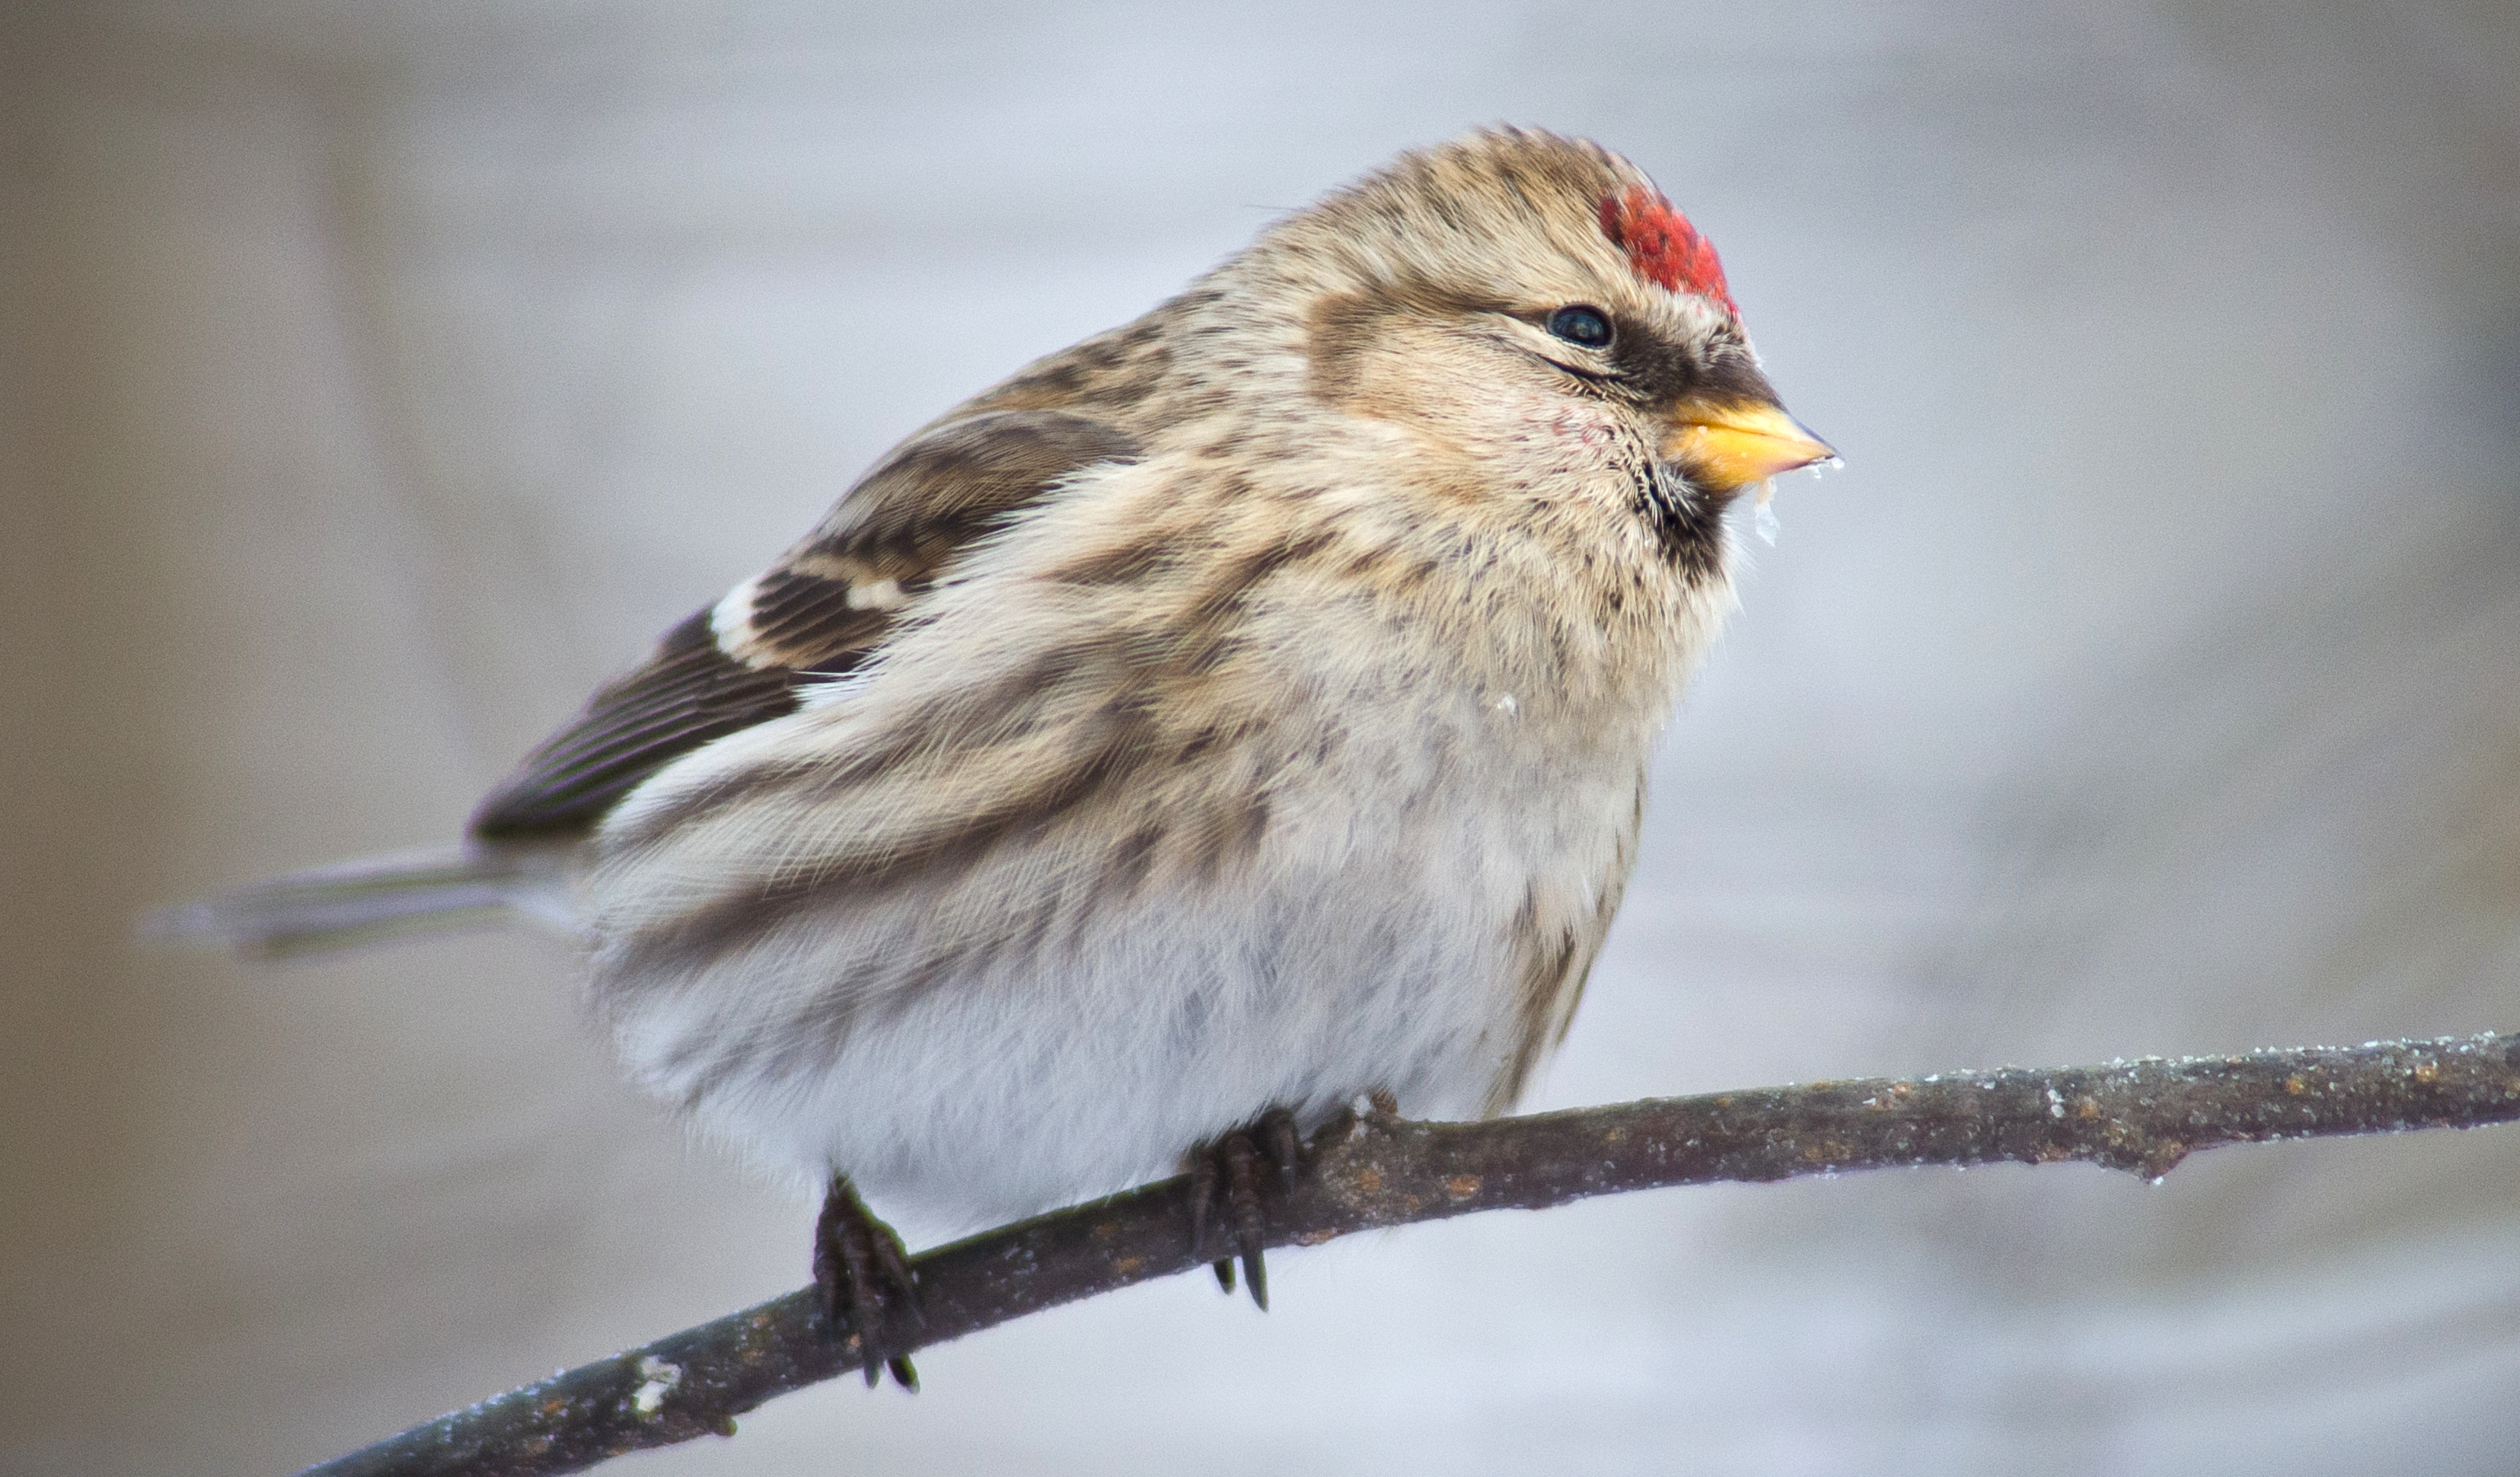
\includegraphics[width=\linewidth]{Acanthis_flammea}
        \caption{A common redpoll (Acanthis Flammea)}
        \label{fig:Acanthis_flammea}
    \end{figure}

\end{center}
\vspace{\baselineskip}

%Students info
\normalsize
\vspace*{\fill}
\begin{flushright}
    Niek R. Scholten (388602)\\
    Bio-Informatics BFV3\\
    Institute of Life Science \& Technology\\
    Hanze University of Applied Sciences\\
    Dave Langers (LADR) \& Bart Barnard (BABA)\\
    \today
\end{flushright}
\newpage

%Blank page
\null
\thispagestyle{empty}
\addtocounter{page}{-1}
\newpage

\begin{center}

%Titles

    \Huge{Predicting bird species from their songs using machine learning}\\
    \vspace{\baselineskip}
    \LARGE{Theme 09 - Introduction Machine Learning}\\
    \vspace{\baselineskip}

\end{center}
\vspace{\baselineskip}

%Students info
\normalsize
\vspace*{\fill}
\begin{flushright}
    Niek R. Scholten (388602)\\
    Bio-Informatics BFV3\\
    Institute of Life Science \& Technology\\
    Hanze University of Applied Sciences\\
    Dave Langers (LADR) \& Bart Barnard (BABA)\\
    \today
\end{flushright}
\newpage

\pagenumbering{roman}
\section*{Abstract}

Here goes the abstract.

\label{sec:abstract}~\addcontentsline{toc}{section}{\nameref{sec:abstract}}
\newpage

\section*{Summary}

Here goes the summary.

\label{sec:summ}~\addcontentsline{toc}{section}{\nameref{sec:summ}}
\newpage

\section*{List of Abbreviations}

\textbf{TEST} Test abbreviation.

\label{sec:abvs}~\addcontentsline{toc}{section}{\nameref{sec:abvs}}

\newpage